% Porto Seguro Safe Driver Prediction - project presentation
% B3155 Project Work in Machine Learning and Data Mining, University of Bologna
% Compile with: latexmk -pdf presentation.tex   (or pdflatex twice)

\documentclass[aspectratio=169,11pt]{beamer}

\usepackage[T1]{fontenc}
\usepackage[utf8]{inputenc}
\usepackage{lmodern}
\usepackage{booktabs}
\usepackage{graphicx}
\usepackage{tikz}
\usetikzlibrary{positioning,arrows.meta,calc}
\graphicspath{{figures/}}

% ------------------------------------------------------------------ look
\definecolor{accent}{RGB}{187,46,41}      % dark red
\definecolor{darkgrey}{RGB}{60,60,60}
\definecolor{lightgrey}{RGB}{242,242,242}
\definecolor{good}{RGB}{31,119,180}

\usetheme{default}
\setbeamercolor{frametitle}{fg=white,bg=accent}
\setbeamercolor{title}{fg=accent}
\setbeamercolor{structure}{fg=accent}
\setbeamercolor{normal text}{fg=darkgrey}
\setbeamercolor{block title}{fg=white,bg=accent}
\setbeamercolor{block body}{bg=lightgrey}
\setbeamerfont{frametitle}{size=\large,series=\bfseries}
\setbeamerfont{title}{size=\Large,series=\bfseries}
\setbeamertemplate{navigation symbols}{}
\setbeamertemplate{itemize items}{\small$\blacktriangleright$}
\setbeamertemplate{frametitle}{%
  \nointerlineskip
  \begin{beamercolorbox}[wd=\paperwidth,ht=2.4ex,dp=1.2ex,leftskip=1em]{frametitle}
    \usebeamerfont{frametitle}\insertframetitle
  \end{beamercolorbox}}
\setbeamertemplate{footline}{%
  \hfill\textcolor{gray}{\scriptsize Porto Seguro Safe Driver Prediction \quad \insertframenumber/\inserttotalframenumber}\hspace{1em}\vspace{0.6em}}

\newcommand{\feat}[1]{\texttt{\small #1}}   % feature names
\newcommand{\hl}[1]{\textcolor{accent}{\textbf{#1}}}

% ------------------------------------------------------------------ title
\title{Porto Seguro Safe Driver Prediction}
\subtitle{Predicting car insurance claims with an ensemble of classifiers}
\author{Lars St\"utzle}
\institute{B3155 Project Work in Machine Learning and Data Mining\\
           Prof.\ Claudio Sartori -- University of Bologna}
\date{A.Y.\ 2026/2027}

\begin{document}

% ================================================================== 1
\begin{frame}[plain]
  \titlepage
  \vfill
  \centering\scriptsize Code and notebooks: \url{https://github.com/lars-stuetzle/stutzle-safedriverprediction}
\end{frame}

% ================================================================== 2
\begin{frame}{Problem and goal}
  \begin{columns}[T]
    \begin{column}{0.55\textwidth}
      \textbf{Business problem}
      \begin{itemize}
        \item Porto Seguro, a Brazilian car insurer, wants to estimate the probability that a driver files a
              claim in the next year
        \item Better estimates $\Rightarrow$ fairer prices: safe drivers pay less, risky drivers pay more
      \end{itemize}
      \medskip
      \textbf{Data mining task}
      \begin{itemize}
        \item Binary classification with probability output (\feat{target} = 1: claim filed)
        \item Kaggle competition (2017)
        \item Only the Kaggle \feat{train.csv} is used (the Kaggle test set has no labels)
      \end{itemize}
    \end{column}
    \begin{column}{0.42\textwidth}
      \begin{block}{Objectives}
        \begin{enumerate}
          \item Understand the data and its quality issues
          \item Leakage-free preparation pipelines
          \item Compare the classifiers of the course
          \item Tune and combine the best models
          \item Evaluate once on held-out data
          \item Interpret the result for the insurer
        \end{enumerate}
      \end{block}
    \end{column}
  \end{columns}
\end{frame}

% ================================================================== 3
\begin{frame}{The data at a glance}
  \begin{columns}[T]
    \begin{column}{0.5\textwidth}
      \begin{itemize}
        \item \hl{595,212} policies, \hl{57} anonymized features
        \item Feature groups by name prefix, types by suffix:
      \end{itemize}
      \medskip
      \centering\footnotesize
      \begin{tabular}{lrrrr}
        \toprule
        group & binary & categ. & numeric & total \\
        \midrule
        \feat{ind} (driver) & 11 & 3 & 4 & 18 \\
        \feat{car}          & 0 & 11 & 5 & 16 \\
        \feat{reg} (region) & 0 & 0 & 3 & 3 \\
        \feat{calc}         & 6 & 0 & 14 & 20 \\
        \midrule
        total & 17 & 14 & 26 & 57 \\
        \bottomrule
      \end{tabular}
    \end{column}
    \begin{column}{0.46\textwidth}
      \textbf{Three challenges}
      \begin{enumerate}
        \item \hl{Class imbalance:} only 3.64\% of the drivers claim (1 in 27)
        \item \hl{Missing values} coded as $-1$ in 12 columns, up to 69\% of a column
        \item \hl{Weak signal:} no single feature separates the classes well
      \end{enumerate}
      \medskip
      No duplicates; the meaning of the features is unknown (anonymized).
    \end{column}
  \end{columns}
\end{frame}

% ================================================================== 4
\begin{frame}{Evaluation protocol and metric}
  \centering
  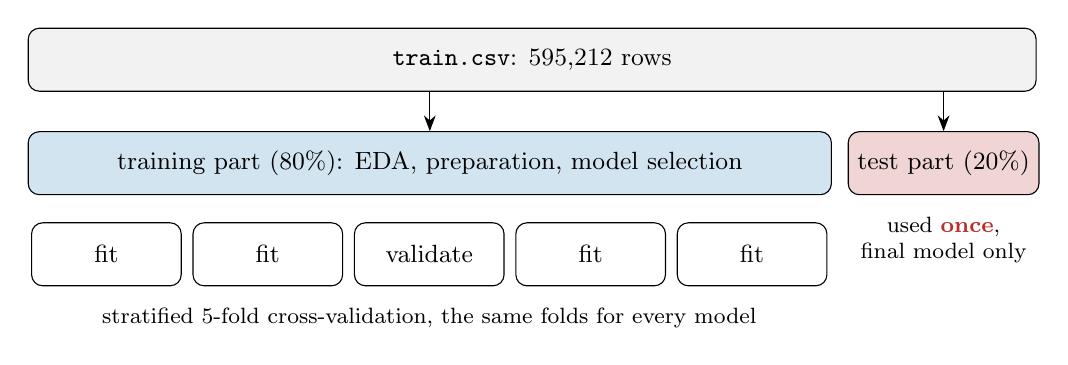
\begin{tikzpicture}[box/.style={draw,rounded corners,minimum height=0.8cm,align=center,font=\small},
                      >={Stealth[length=2mm]}]
    \node[box,fill=lightgrey,minimum width=12.8cm] (all) {\feat{train.csv}: 595,212 rows};
    \node[box,fill=good!20,minimum width=10.2cm,below=0.5cm of all.south west,anchor=north west] (train)
      {training part (80\%): EDA, preparation, model selection};
    \node[box,fill=accent!20,minimum width=2.4cm,right=0.2cm of train] (test) {test part (20\%)};
    \foreach \i in {1,...,5} {
      \node[box,minimum width=1.9cm,fill=white] at ($(train.south west)+(1.0+2.05*\i-2.05,-0.75)$) (f\i)
        {\ifnum\i=3 validate\else fit\fi};
    }
    \node[font=\footnotesize,below=0.15cm of f3] {stratified 5-fold cross-validation, the same folds for every model};
    \node[font=\footnotesize,below=0.15cm of test,align=center] {used \hl{once},\\final model only};
    \draw[->] (all.south -| train.north) -- (train.north);
    \draw[->] (all.south -| test.north) -- (test.north);
  \end{tikzpicture}

  \vspace{0.2cm}
  \begin{columns}[T]
    \begin{column}{0.48\textwidth}
      \textbf{Main metric: normalized Gini} (competition metric)
      \[ \text{Gini} = 2\cdot\text{AUC} - 1 \]
      Depends only on the \emph{ranking} of the drivers; 0 = random, 1 = perfect.
    \end{column}
    \begin{column}{0.48\textwidth}
      \textbf{Why not accuracy?}
      Always predicting ``no claim'' gives \hl{96.4\%} accuracy and is useless.
      Also reported: PR-AUC (focus on the rare class) and the train Gini (overfitting).
    \end{column}
  \end{columns}
\end{frame}

% ================================================================== 5
\begin{frame}{EDA (1): missing values carry information}
  \begin{columns}[T]
    \begin{column}{0.52\textwidth}
      \centering\small
      \begin{tabular}{lrrr}
        \toprule
        column & missing & \multicolumn{2}{c}{claim rate} \\
               &         & missing & present \\
        \midrule
        \feat{ps\_car\_03\_cat} & 69.1\% & 3.3\% & 4.5\% \\
        \feat{ps\_car\_05\_cat} & 44.8\% & 3.2\% & 4.0\% \\
        \feat{ps\_reg\_03}      & 18.1\% & 2.8\% & 3.8\% \\
        \feat{ps\_car\_07\_cat} & 1.9\%  & \hl{7.8\%} & 3.6\% \\
        \feat{ps\_ind\_05\_cat} & 1.0\%  & \hl{8.0\%} & 3.6\% \\
        \feat{ps\_car\_01\_cat} & 84 rows & \hl{29.8\%} & 3.6\% \\
        \bottomrule
      \end{tabular}
    \end{column}
    \begin{column}{0.45\textwidth}
      \begin{itemize}
        \item Depending on the column, a missing value means a \hl{lower} or a \hl{much higher} risk
        \item Dropping rows would remove most of the data; dropping columns would lose signal
      \end{itemize}
      \begin{block}{Decision}
        Keep ``missing'' as information: own category for categorical features, a 0/1 indicator for
        numeric ones, native NaN support in tree models.
      \end{block}
    \end{column}
  \end{columns}
\end{frame}

% ================================================================== 6
\begin{frame}{EDA (2): many weak features, and 20 pure-noise features}
  \centering
  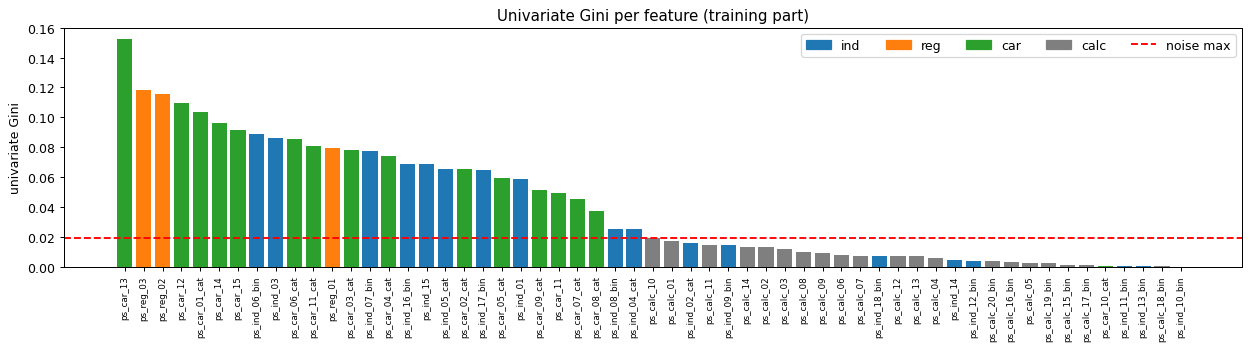
\includegraphics[width=\textwidth]{eda_univariate_gini.png}
  \begin{itemize}
    \item Best single feature: \feat{ps\_car\_13} with Gini 0.15; the signal is spread over many weak features
    \item All 20 \feat{calc} features are below the best of 20 \hl{random noise} columns (red line)
    \item Redundancies: \feat{ps\_ind\_14} = sum of \feat{ps\_ind\_10..13\_bin}; near-constant features (> 99\% one value)
  \end{itemize}
\end{frame}

% ================================================================== 7
\begin{frame}{Data preparation: two pipelines}
  \begin{columns}[T]
    \begin{column}{0.48\textwidth}
      \begin{block}{Linear models (LR, Naive Bayes, MLP)}
        \small
        \begin{itemize}
          \item numeric: median imputation + missing indicator, standardization
          \item categorical: ``missing'' category, one-hot encoding, rare categories ($<$ 500 rows) grouped
          \item binary: unchanged; \feat{ps\_ind\_14} dropped
          \item 57 $\rightarrow$ 227 columns, sparse (20\% non-zero)
        \end{itemize}
      \end{block}
    \end{column}
    \begin{column}{0.48\textwidth}
      \begin{block}{Tree models (tree, RF, boosting)}
        \small
        \begin{itemize}
          \item no imputation, scaling or encoding
          \item NaN and categorical features handled natively
          \item only column selection
        \end{itemize}
      \end{block}
    \end{column}
  \end{columns}
  \vspace{0.2cm}
  \small
  \begin{itemize}
    \item Every step is a scikit-learn \texttt{Pipeline} / \texttt{ColumnTransformer}: it is \hl{refitted inside
          every CV fold}, so no information leaks from the validation fold
    \item Shared code in \texttt{src/} (loading, split, pipelines, evaluation, final model)
  \end{itemize}
\end{frame}

% ================================================================== 8
\begin{frame}{Models compared}
  \begin{columns}[T]
    \begin{column}{0.5\textwidth}
      \textbf{Baselines}
      \begin{itemize}
        \item Dummy (constant claim rate): Gini 0
        \item Default logistic regression: 0.257
        \item Default gradient boosting: 0.253 (train 0.41 $\Rightarrow$ overfitting)
      \end{itemize}
      \medskip
      \textbf{Single classifiers}
      \begin{itemize}
        \item Logistic regression (grid over $C$)
        \item Decision tree (depth $\times$ leaf size)
        \item Gaussian Naive Bayes
        \item MLP neural network (2 sizes)
      \end{itemize}
    \end{column}
    \begin{column}{0.48\textwidth}
      \textbf{Ensembles}
      \begin{itemize}
        \item Random forest (bagging), tuned with the \hl{out-of-bag} estimate
        \item Histogram gradient boosting, \hl{randomized search} (20 configurations, early stopping)
        \item Soft voting of the three best families
      \end{itemize}
      \medskip
      \textbf{Not used}
      \begin{itemize}
        \item kNN: slow prediction, distances meaningless in 227 mostly one-hot dimensions
        \item Kernel SVM: training time quadratic to cubic in 476k rows
      \end{itemize}
    \end{column}
  \end{columns}
\end{frame}

% ================================================================== 9
\begin{frame}{Controlling overfitting}
  \begin{columns}[c]
    \begin{column}{0.55\textwidth}
      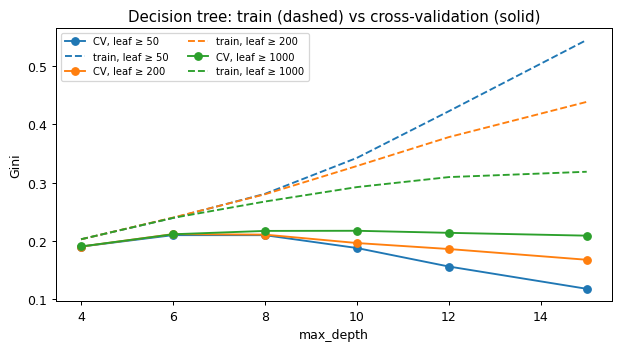
\includegraphics[width=\textwidth]{tree_depth_overfitting.png}
    \end{column}
    \begin{column}{0.43\textwidth}
      \textbf{Decision tree}
      \begin{itemize}
        \item Deeper trees: train Gini up to 0.54, CV Gini down to 0.12
        \item Large leaves (1000 rows) act as regularization
        \item Best tree: only 0.217
      \end{itemize}
      \textbf{Logistic regression}
      \begin{itemize}
        \item Train and CV differ by only 0.01 for every $C$: \hl{no overfitting}, limited by bias
      \end{itemize}
      \textbf{Gradient boosting}
      \begin{itemize}
        \item Tuning: slow learning rate, small trees, large leaves $\Rightarrow$ train Gini 0.41 $\rightarrow$ 0.36,
              CV 0.253 $\rightarrow$ 0.266
      \end{itemize}
    \end{column}
  \end{columns}
\end{frame}

% ================================================================== 10
\begin{frame}{What did \emph{not} help}
  \centering
  \begin{tabular}{llrr}
    \toprule
    experiment & model & CV Gini before & after \\
    \midrule
    remove the 20 \feat{calc} features & logistic regression & 0.2573 & 0.2582 \\
                                       & gradient boosting   & 0.2525 & 0.2522 \\
    \midrule
    balanced class weights & logistic regression & 0.2592 & 0.2588 \\
                           & gradient boosting   & 0.2660 & 0.2647 \\
    \midrule
    new feature \feat{n\_missing} & logistic regression & 0.2592 & 0.2592 \\
                                  & gradient boosting   & 0.2660 & 0.2667 \\
    \bottomrule
  \end{tabular}

  \vspace{0.5cm}
  \begin{itemize}
    \item All changes are far below the fold-to-fold standard deviation (0.005 -- 0.010)
    \item \feat{calc} features \hl{removed} anyway (simpler, faster; confirms the EDA) $\Rightarrow$ 37 features
    \item Class weights do not improve a \emph{ranking} metric; the imbalance is handled by the metric choice
          and the threshold
  \end{itemize}
\end{frame}

% ================================================================== 11
\begin{frame}{Model comparison (5-fold CV on the training part)}
  \begin{columns}[c]
    \begin{column}{0.58\textwidth}
      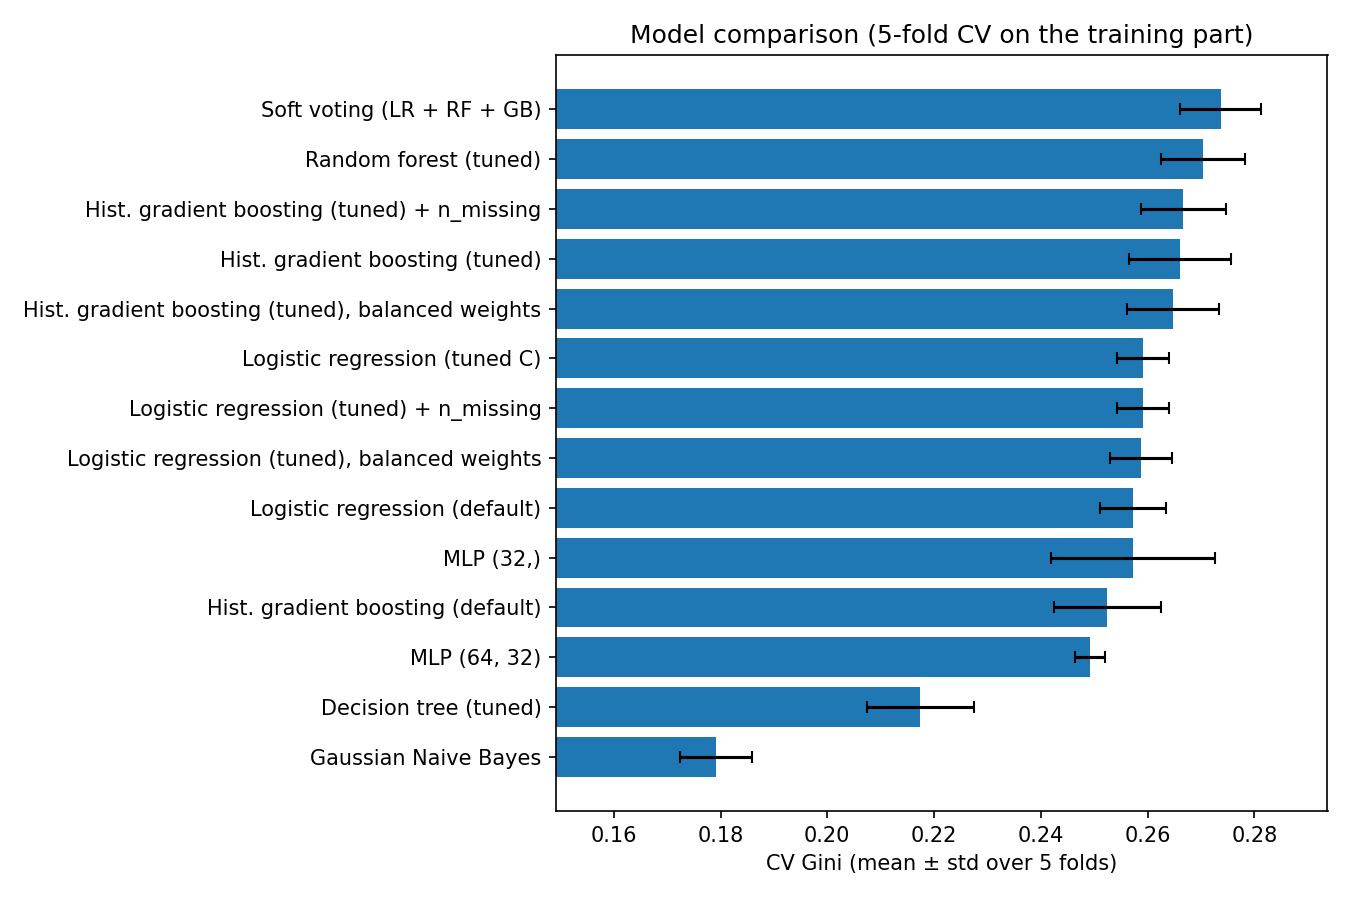
\includegraphics[width=\textwidth]{03_model_comparison.png}
    \end{column}
    \begin{column}{0.4\textwidth}
      \small
      \begin{itemize}
        \item \hl{Ensembles are best}: random forest 0.270, gradient boosting 0.266
        \item MLP and Naive Bayes do not beat logistic regression
        \item \hl{Soft voting} (LR + RF + GB): CV Gini \hl{0.274}, best PR-AUC (0.066)
        \item Different model families make different errors $\Rightarrow$ averaging reduces variance
      \end{itemize}
      \begin{block}{Final model}
        Soft voting of tuned LR, RF and GB
      \end{block}
    \end{column}
  \end{columns}
\end{frame}

% ================================================================== 12
\begin{frame}{Final evaluation on the held-out test part}
  \begin{columns}[c]
    \begin{column}{0.53\textwidth}
      \centering\footnotesize
      \begin{tabular}{lccc}
        \toprule
        model & CV Gini & test Gini & 95\% CI \\
        \midrule
        \textbf{Soft voting} & 0.274 & \hl{0.281} & 0.265 -- 0.298 \\
        Gradient boosting & 0.266 & 0.278 & 0.261 -- 0.295 \\
        Random forest & 0.270 & 0.271 & 0.254 -- 0.288 \\
        Logistic regression & 0.259 & 0.267 & 0.250 -- 0.284 \\
        \bottomrule
      \end{tabular}

      \bigskip
      \begin{itemize}
        \item 119,043 unseen drivers, 4,339 claims
        \item Test scores agree with the CV estimates: \hl{no winner's curse}
        \item 95\% CI from 1,000 bootstrap samples
      \end{itemize}
    \end{column}
    \begin{column}{0.45\textwidth}
      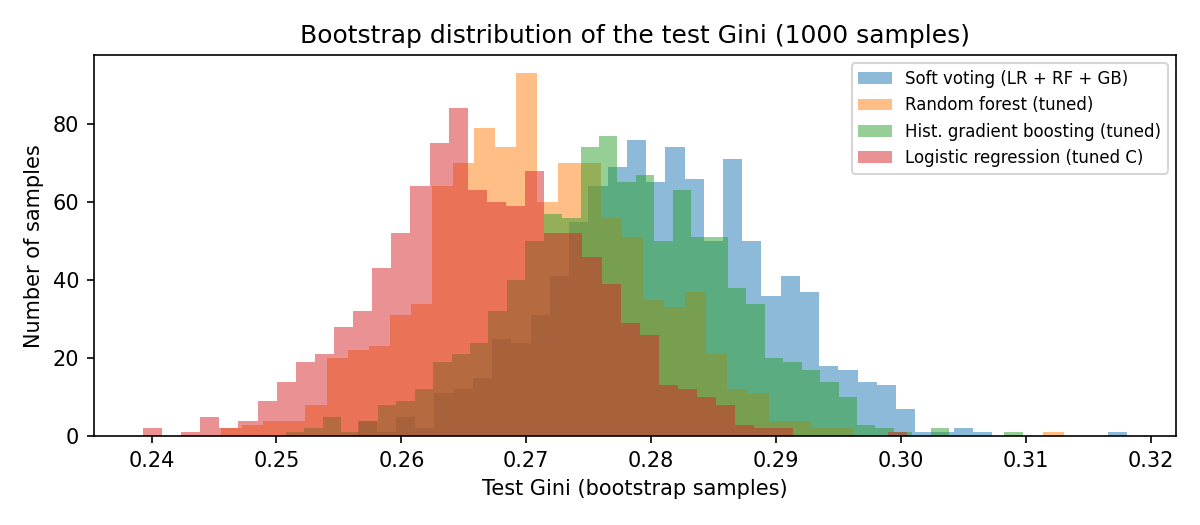
\includegraphics[width=\textwidth]{04_bootstrap.png}
      \small\textbf{Paired bootstrap} (same resampled drivers): the ensemble beats the random forest and the
      logistic regression in \hl{100\%} of the samples, gradient boosting in 94\%.
    \end{column}
  \end{columns}
\end{frame}

% ================================================================== 13
\begin{frame}{ROC and precision-recall curves (test part)}
  \centering
  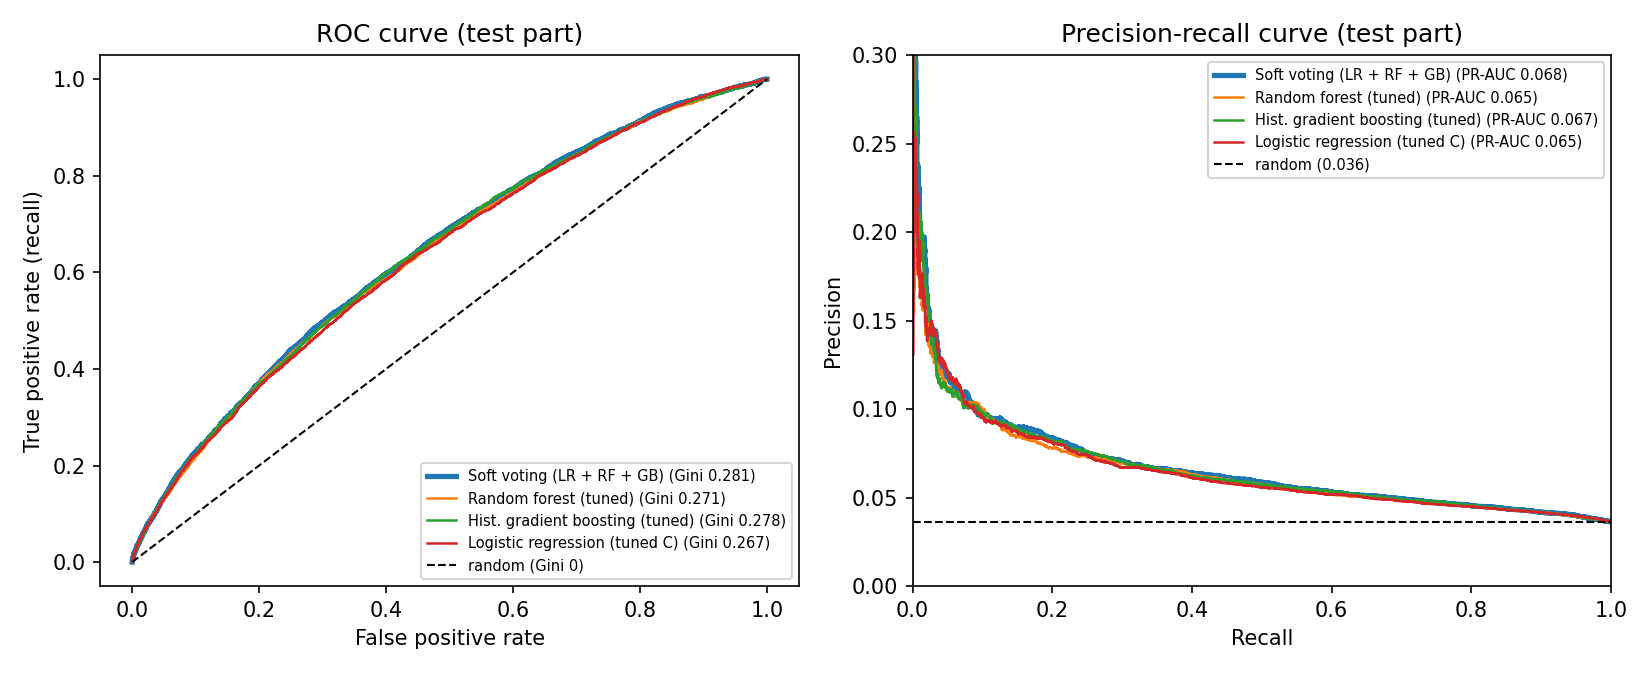
\includegraphics[width=0.9\textwidth]{04_roc_pr.png}
  \begin{itemize}
    \item The four models are close; all clearly above random
    \item Precision falls quickly: about 8\% at a recall of 20\% (random: 3.6\%) $\Rightarrow$ the model shifts
          the odds, it cannot \emph{identify} single claimants
  \end{itemize}
\end{frame}

% ================================================================== 14
\begin{frame}{Lift, calibration and cumulative gains}
  \centering
  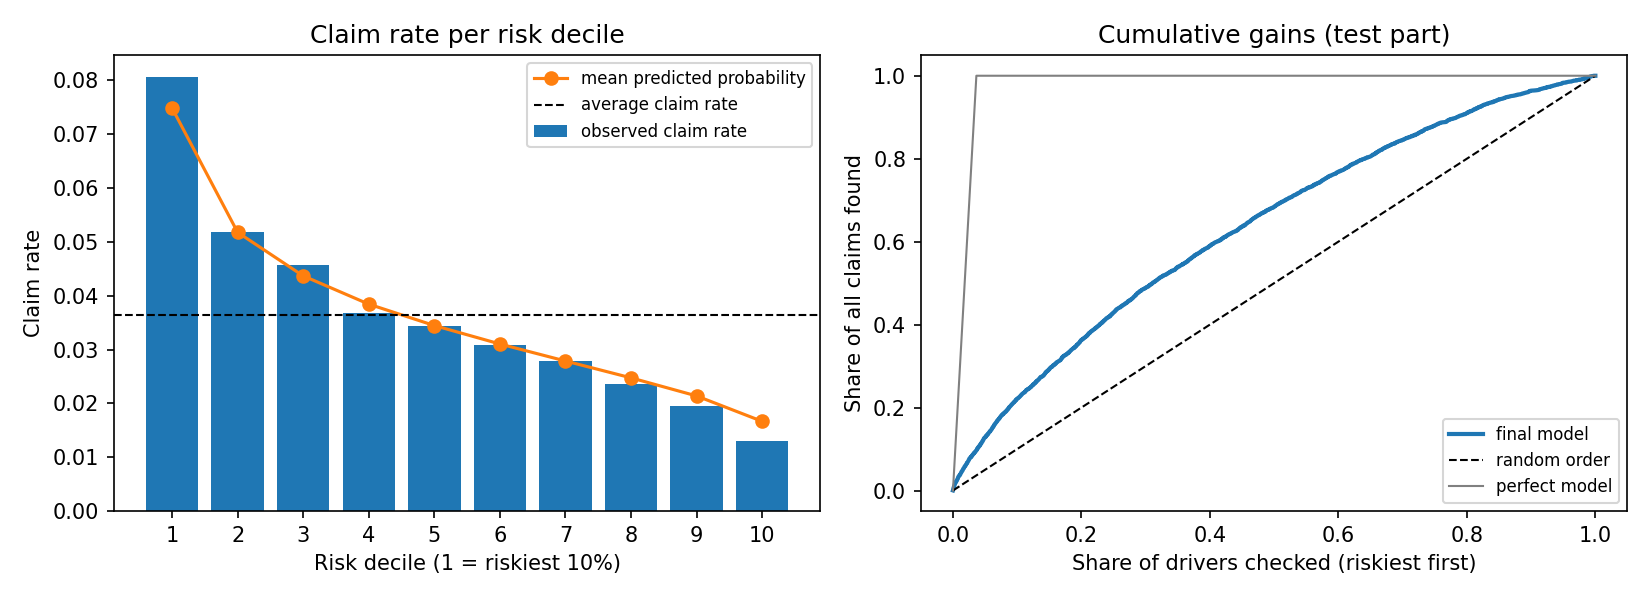
\includegraphics[width=0.9\textwidth]{04_lift_gains.png}
  \begin{itemize}
    \item Riskiest 10\%: claim rate \hl{8.1\%} (lift 2.2), safest 10\%: \hl{1.3\%} $\Rightarrow$ factor 6
    \item Predicted and observed rates agree in every decile ($\pm$ 0.6 pp): the probabilities are \hl{calibrated}
    \item The riskiest 30\% of the drivers account for 49\% of all claims
  \end{itemize}
\end{frame}

% ================================================================== 15
\begin{frame}{Decision threshold}
  Thresholds chosen on \hl{out-of-fold predictions of the training part}, then applied to the test part:

  \medskip
  \centering\small
  \begin{tabular}{lrrrrrr}
    \toprule
    threshold & flagged & true pos. & false pos. & precision & recall & accuracy \\
    \midrule
    0.5 (default)       & 0\%    & 0   & 0      & --    & 0\%   & 96.4\% \\
    max F1: 0.058       & 9.8\%  & 948 & 10,742 & 8.1\% & 21.9\% & 88.1\% \\
    riskiest 10\%: 0.0575 & 10.3\% & 976 & 11,265 & 8.0\% & 22.5\% & 87.7\% \\
    \bottomrule
  \end{tabular}

  \medskip
  \raggedright
  \begin{itemize}
    \item No driver reaches a claim probability of 50\%: the default threshold flags \hl{nobody}
    \item Flagging the riskiest 10\%: precision 2.2$\times$ the claim rate, but about 12 false alarms per claimant
    \item Best F1 only 0.12 $\Rightarrow$ the model is a \hl{risk score}, not a yes/no classifier
  \end{itemize}
\end{frame}

% ================================================================== 16
\begin{frame}{Which features matter? (permutation importance, test part)}
  \begin{columns}[c]
    \begin{column}{0.66\textwidth}
      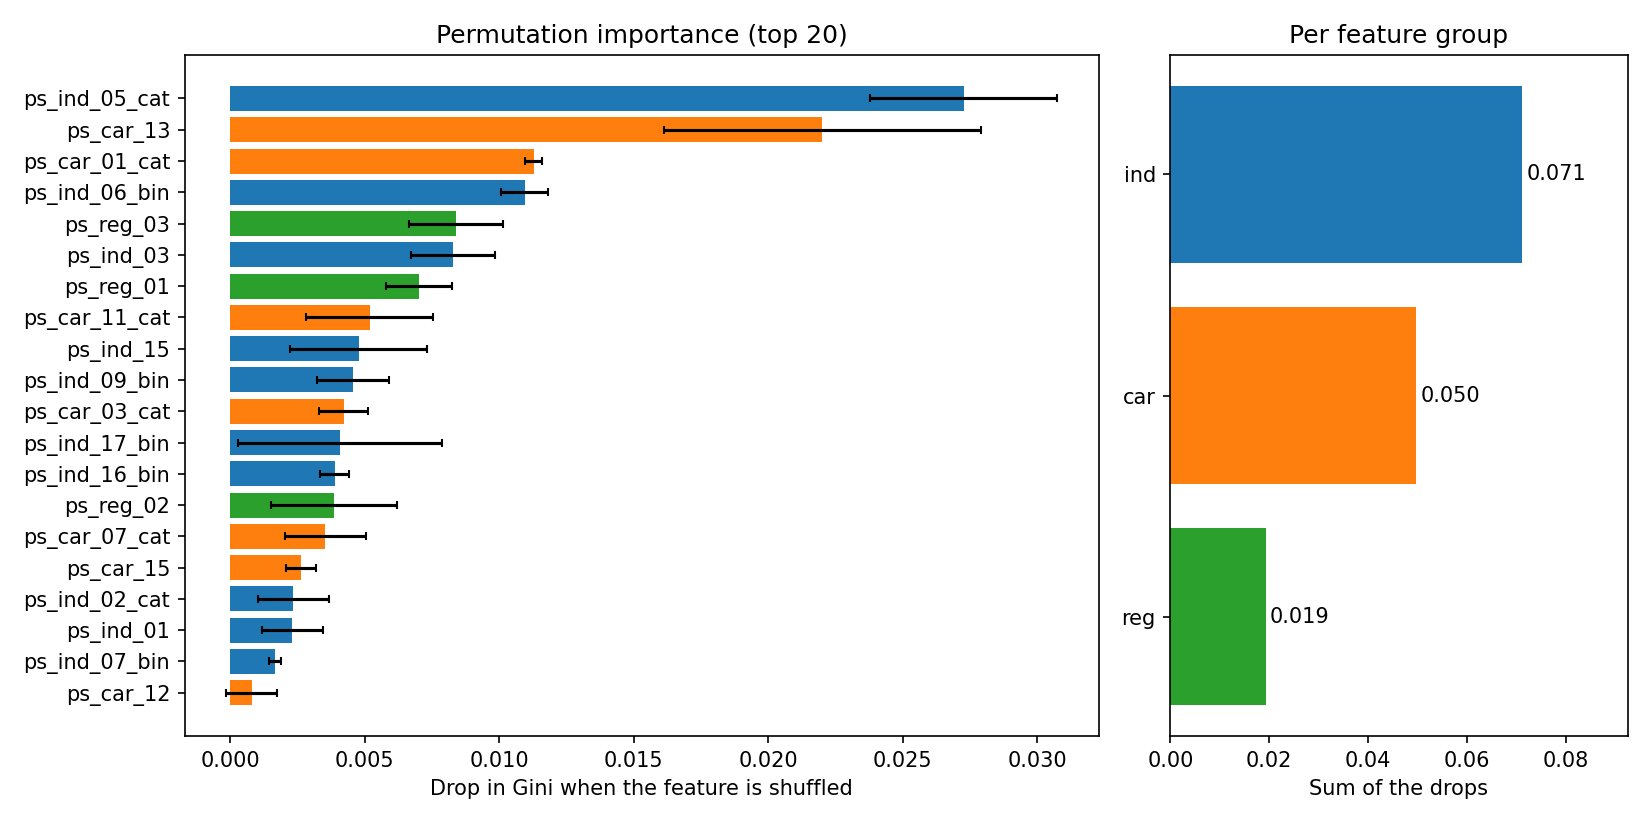
\includegraphics[width=\textwidth]{04_permutation_importance.png}
    \end{column}
    \begin{column}{0.32\textwidth}
      \small
      \begin{itemize}
        \item Shuffle one feature, measure the drop in Gini
        \item Top: \feat{ps\_ind\_05\_cat}, \feat{ps\_car\_13} (also strongest in the EDA)
        \item \feat{ps\_car\_01\_cat}: signal from its missing values $\Rightarrow$ keeping ``missing'' paid off
        \item Near-constant features from the EDA: importance $\approx 0$
        \item Driver features (\feat{ind}) contribute most in total
      \end{itemize}
    \end{column}
  \end{columns}
\end{frame}

% ================================================================== 17
\begin{frame}{Interpretation for the insurer}
  \begin{columns}[T]
    \begin{column}{0.48\textwidth}
      \begin{block}{Use}
        \begin{itemize}
          \item \textbf{Pricing:} premium (frequency part) proportional to the predicted probability:
                riskiest decile about 2.2$\times$, safest about 0.4$\times$ the average
          \item \textbf{Targeting:} reviewing or offering telematics to the riskiest 30\% reaches half of
                all future claims
        \end{itemize}
      \end{block}
    \end{column}
    \begin{column}{0.48\textwidth}
      \begin{block}{Limits}
        \begin{itemize}
          \item Predicts \emph{whether} a claim happens, not its \emph{cost}
          \item 92\% of the riskiest decile do not claim: no individual decisions based on the model alone
          \item Anonymized features: check for proxies of protected attributes (fairness)
          \item One time period: monitor and refit when the portfolio changes
        \end{itemize}
      \end{block}
    \end{column}
  \end{columns}
\end{frame}

% ================================================================== 18
\begin{frame}{Conclusions}
  \begin{enumerate}
    \item Following CRISP-DM, every decision (feature removal, tuning, model choice, threshold) was made on the
          \hl{training part only}; the test part was used once
    \item Final model: \hl{soft voting} of logistic regression, random forest and gradient boosting,
          test Gini \hl{0.281} (95\% CI 0.265 -- 0.298), in line with the CV estimate (0.274)
    \item Ensembles gave the main improvement over the baseline (0.257 $\rightarrow$ 0.281); feature removal,
          class weights and a missing-count feature did not
    \item Claims are hard to predict for one driver, but drivers can be \hl{ranked} well: a factor of 6 between
          the riskiest and the safest decile, with calibrated probabilities
  \end{enumerate}
  \smallskip
  \textbf{Possible next steps}
  \small
  \begin{itemize}
    \item Target encoding of the high-cardinality \feat{ps\_car\_11\_cat}; other boosting libraries (LightGBM, XGBoost)
    \item Comparison on Kaggle's own test set with a late submission (winning private score: about 0.297)
  \end{itemize}
\end{frame}

% ================================================================== appendix
\appendix
\begin{frame}{References}
  \small
  \begin{itemize}
    \item Porto Seguro's Safe Driver Prediction, Kaggle competition, 2017.\\
          \url{https://www.kaggle.com/competitions/porto-seguro-safe-driver-prediction}
    \item C.\ Sartori, \emph{Machine Learning and Data Mining}, lecture slides, University of Bologna, 2026.
    \item P.\ Chapman et al., \emph{CRISP-DM 1.0: Step-by-step data mining guide}, SPSS, 2000.
    \item F.\ Pedregosa et al., \emph{Scikit-learn: Machine Learning in Python}, JMLR 12, pp.\ 2825--2830, 2011.
    \item P.-N.\ Tan, M.\ Steinbach, V.\ Kumar, \emph{Introduction to Data Mining}, Addison Wesley, 2006.
  \end{itemize}
  \vfill
  \centering
  Code, notebooks and results: \url{https://github.com/lars-stuetzle/stutzle-safedriverprediction}
\end{frame}

\end{document}
